\documentclass[xcolor=svgnames,dvipsnames,table, hyperref=pdftex, mathserif, presentation]{beamer}
\usepackage{amsmath,amssymb,amsfonts,amsthm}
\usepackage{ctex}
\usepackage{graphics}
\usepackage{graphicx}
\usepackage{xcolor}
\usepackage{wasysym}
\usepackage{bbm}
\usepackage{url}
\usepackage{beamerleanprogress}
\usepackage{tikz-dependency}
\usepackage{tikz-qtree}

\usetheme{CambridgeUS}
%\usetheme{Pittsburgh}
\usecolortheme{orchid} % seahorse  orchid rose
\setbeamertemplate{blocks}[rounded][shadow=true]
\AtBeginSection[]{%
  \begin{frame}<beamer>
    \frametitle{Outline}
      \tableofcontents[current] 
    \end{frame}
  \addtocounter{framenumber}{-1}% If you don't want them to affect the slide number
}
\AtBeginSubsection[]
{
  \begin{frame}
  \frametitle{Outline}
    \tableofcontents[currentsection,currentsubsection]
  %\tableofcontents[sectionstyle=show/hide,subsectionstyle=hide/show/hide]
  \end{frame}
  \addtocounter{framenumber}{-1}% If you don't want them to affect the slide number
}
\newcommand{\setof}[1]{\ensuremath{\left \{ #1 \right \}}}
\newcommand{\tuple}[1]{\ensuremath{\left \langle #1 \right \rangle }}
\newcommand{\red}[1]{\textcolor{red}{#1}}
\newcommand{\brown}[1]{\textcolor{brown}{#1}}
\newcommand{\green}[1]{\textcolor{green}{#1}}
\newcommand{\blue}[1]{\textcolor{blue}{#1}}
\newcommand{\cyan}[1]{\textcolor{cyan}{#1}}

%gets rid of navigation symbols
\setbeamertemplate{navigation symbols}{}

\begin{document}

\title[EMNLP]{Typed Tensor Decomposition of Knowledge Bases For Relation Extration}

\institute[icst@pku]{
  
}
\author[Zhe Han]{Kai-Wei Chang:  University of Illinois \\
    Bishan Yang: Cornell Univer. \\
    Wen-tau Yih, Christopher Meek: Microsoft Research
}

\frame[t,plain]{ \titlepage } % [t,plain]

\frame{
  \frametitle{ Outline  }
  
   \begin{itemize}
  \item RE introduction
  \item Related word(other approch)
  \item background
    \begin{itemize}
    \item Tensor encoding
    \item RESCAL
    \end{itemize}
  \item Approch(improment)
    \begin{itemize}
     \item Domain Knowledge
     \item Reguliation efficiency
    \end{itemize}

  \item  Experiment
    \begin{itemize}
     \item Knowledge base Completion
     \item Relation extraction
    \end{itemize}
  
  \item Conclusions
  \end{itemize}

}

\frame{
  \frametitle{ RE introduction }
  
    \begin{itemize}
    \item Tradition
	\begin{itemize}
	 \item 分类问题,利用文本特征
	 \item 没有利用已有KB的知识帮助判断
	\end{itemize}
    \item Later
	\begin{itemize}
	 \item (collective filtering?)把relation转化为vector,实体对和relation建立关系,映射到相同的vector上,然后计算相似度
	\begin{tabular}{|c|c|c|c|}
	 \hline
	  & $r_1$ & $r_2$ & $r_3$\\ \hline
	  (e1,e2) & 1 & &\\ \hline
	  (e2,e4) &  & 1 &\\ \hline
	  (e1,e3) & 1 & &\\ \hline
	 \end{tabular}
	 \item 没有挖掘entity信息,只是用序号代替entity
	\end{itemize}
    \item TRESCAL
	\begin{itemize}
	 \item 利用relation限制和entity类别来剪枝
	 \item 运行速度快,不影响关系抽取效果
	\end{itemize}

  \end{itemize}
}

\frame{
  \frametitle{Related word(other approch)}
  \begin{itemize}
   \item 张量分解
      \begin{itemize}
       \item CP(可分布式) or Tucker decompositions
       \item triples->tensor;CP decomposotion;extract hidden triples
       \item 改进:加入entity类别信息有关的约束到目标函数中(基于无参的3-way tensor贝叶斯模型)
       \item 大多数TD model空间大,慢不实用
      \end{itemize}
   \item 神经网络
      \begin{itemize}
       \item 1.学习$(e_i, r_k)$的向量表示
       \item 2.对于任意$(e_i, r_k,e_j)$,得到$Vector(e_i,r_k),Vector(e_j,r_k), Score(e_i,r_k,e_j)=v(e_i,r_k)\cdot v(e_j,r_k)$
       \begin{itemize}
        \item $Score(e_i,r_k,e_j)=-\Arrowvert \mathbf{e_i+r_k-e_j}\Arrowvert$
       \end{itemize}

       
      \end{itemize}
   \item 神经网络2
      \begin{itemize}
       \item 1.学习单词的向量vector,每个关系的矩阵R
       \item 2.$Score(e_i,r_k,e_j)=vector(e_i)\mathcal{R}_kvector^T(e_j)$
      \end{itemize}

  \end{itemize}

}
\frame{
  \frametitle{background} 
  \begin{itemize}
   \item triples->tensor
  \begin{figure}[h]
  \centering
  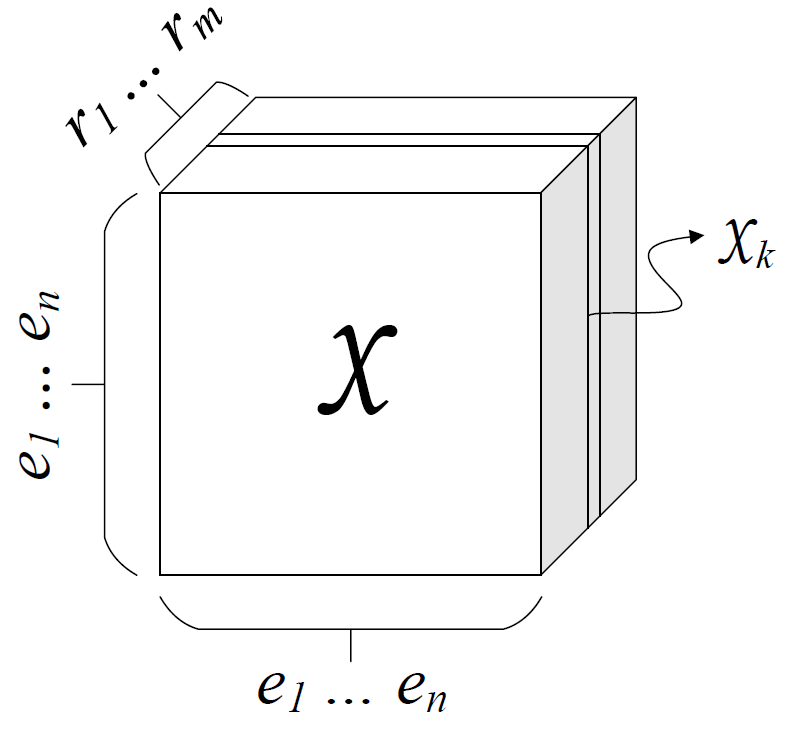
\includegraphics[width=0.2\textwidth]{tensor}
  \end{figure}
   \item $\mathcal{X}_k\thickapprox \mathbf{A}\mathcal{R}_k\mathbf{A^T}$
   \item $[\mathbf{A}]_{n\times r}, [\mathcal{R}_k]_{r\times r}$
  \begin{figure}[h]
  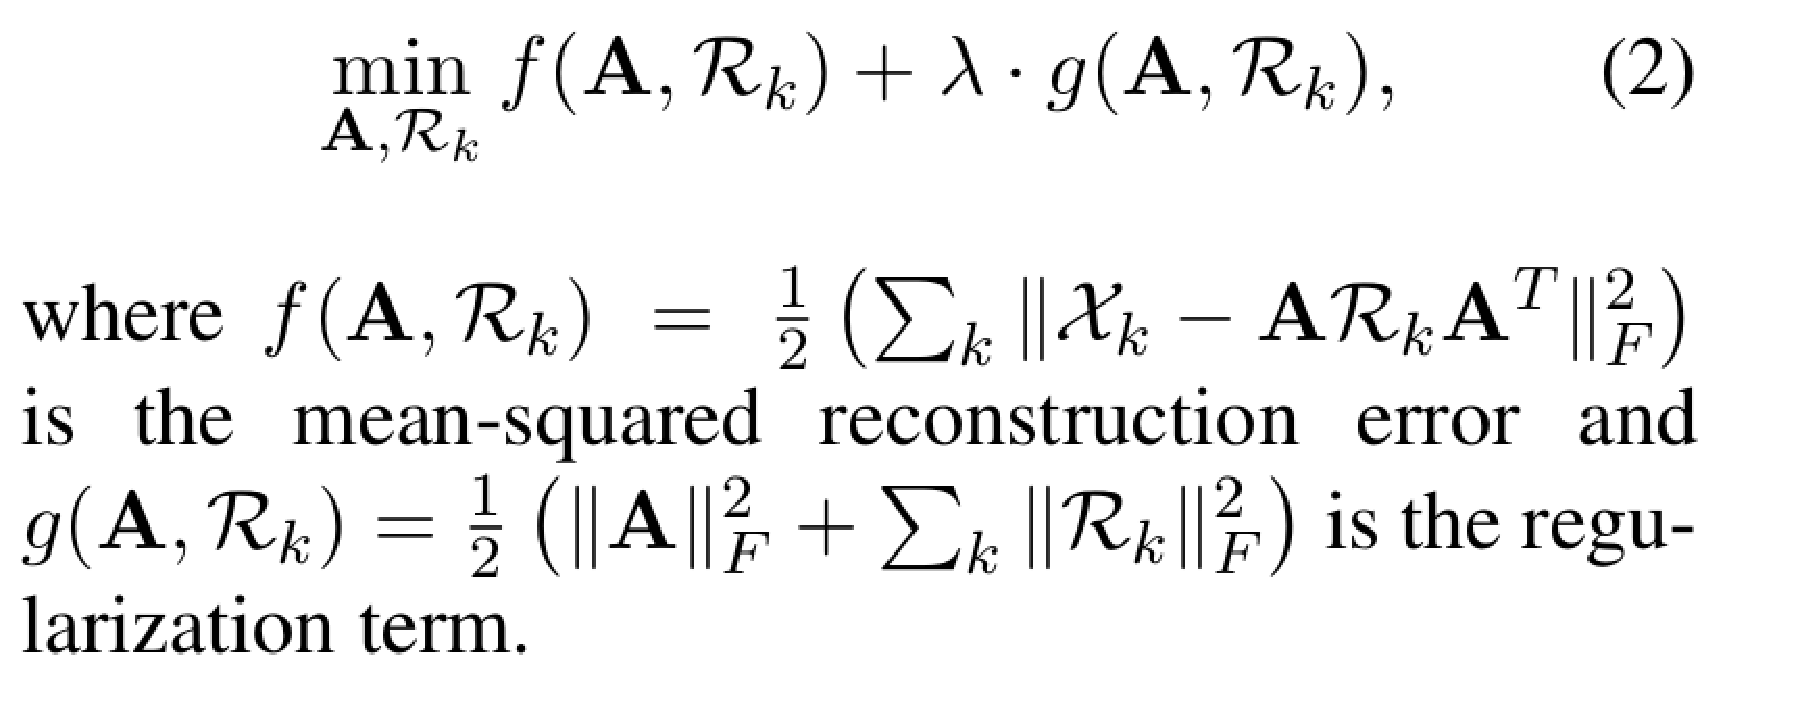
\includegraphics[width=0.6\textwidth]{lossFunc}
  \end{figure}
   \item 优化:交替优化(ALS)
  \end{itemize}
}

\frame{
  \frametitle{Approch (improment)}
  \begin{itemize}
   \item Domain Knowledge,加入类别判断
   \begin{itemize}
    \item (person, born-in, person)剔除
    \item $\mathcal{X},\mathbf{A}$的维数都减少\\
    
  \begin{figure}[h]
  \centering
  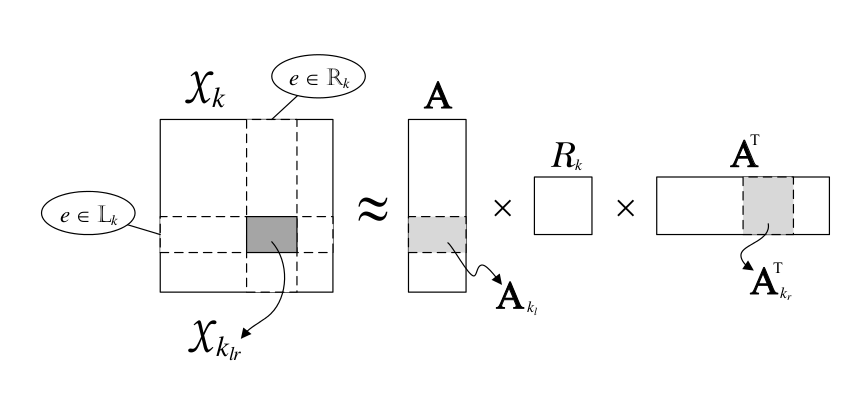
\includegraphics[width=0.5\textwidth]{DomSub}
  \end{figure}
  
   \end{itemize}
   \item SVD分解[p5右中]
      \begin{itemize}
       \item 原来的瓶颈:求$[(\mathbf{Z}^T\mathbf{Z}+\lambda I)^{-1}]_{r^2\times r^2}$[p4左中]
       \item 替代为求$\mathbf{A}_{k_{lr}}$的SVD分解
      \end{itemize}
   \item 速度提升为4倍多
  \end{itemize}
}

\frame{
  \frametitle{Experiment}
  \begin{itemize}
   
   \item KB completion
   \begin{itemize}
    \item NELL:v165(training), v166/533(development), v534/745(test)
    \item Entity etrival:$(e_i,r_k,?)$
    \begin{itemize}
     \item 1个真实答案$e_j$+100个随机挑选的实体$e'_1,...,e'_100$,在其中查找答案
     \item 2.$Score(e_i,r_k,e_j)=(a^T)_iR_ka^j$
    \end{itemize}
   \end{itemize}
   


   \item Relation Retrieval:$(e_i,?,e_j)$
   \begin{itemize}
    \item $Score(e_i,r_k,e_j)=(a^T)_iR_ka^j$, Domain效果不好
    \begin{itemize}
     \item 作者解释:entity类别表错导致准确率降低(直接被筛掉了)
    \end{itemize}
    \item 含有相似relation的relation 比较容易判断出来
	\begin{itemize}
	 \item 上位词,抽象词的关系更容易表示?
	\end{itemize}

   \end{itemize}

  \begin{figure}[h]
  \centering
  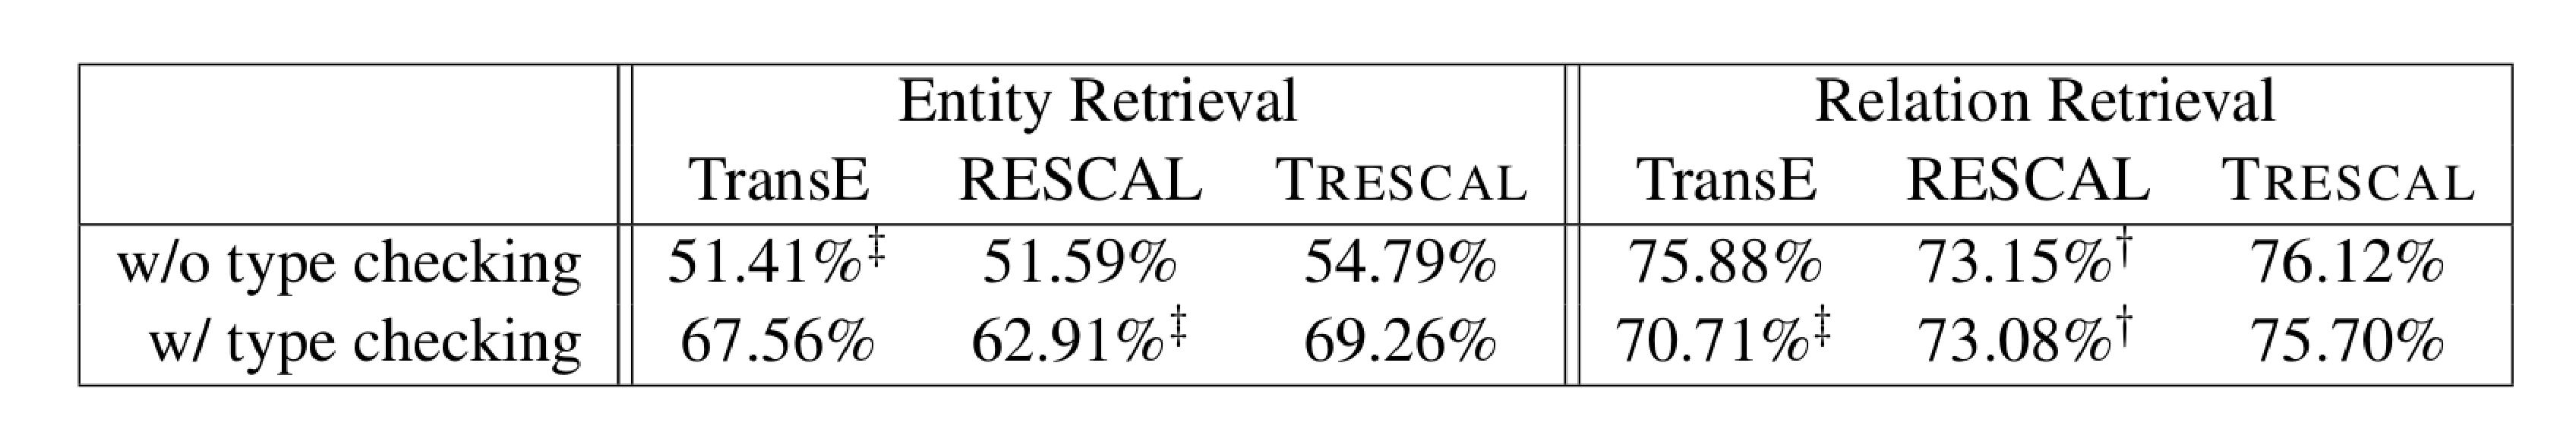
\includegraphics[width=0.8\textwidth]{KBpfm}
  \end{figure}
  \end{itemize}
}

\frame{
  \frametitle{Experiment and Conclusions}
  \begin{itemize}
   \item Relation extraction
   \begin{itemize}
    \item 比如RI13,对于任意relation $r_k$,利用RI13返回的前1000个实体$(e_i,e_j)$对作为候选,取得分最高的前100个作为本系统的输出结果,并比较正确率(发现有明显提高)
    
  \begin{figure}[h]
  \centering
  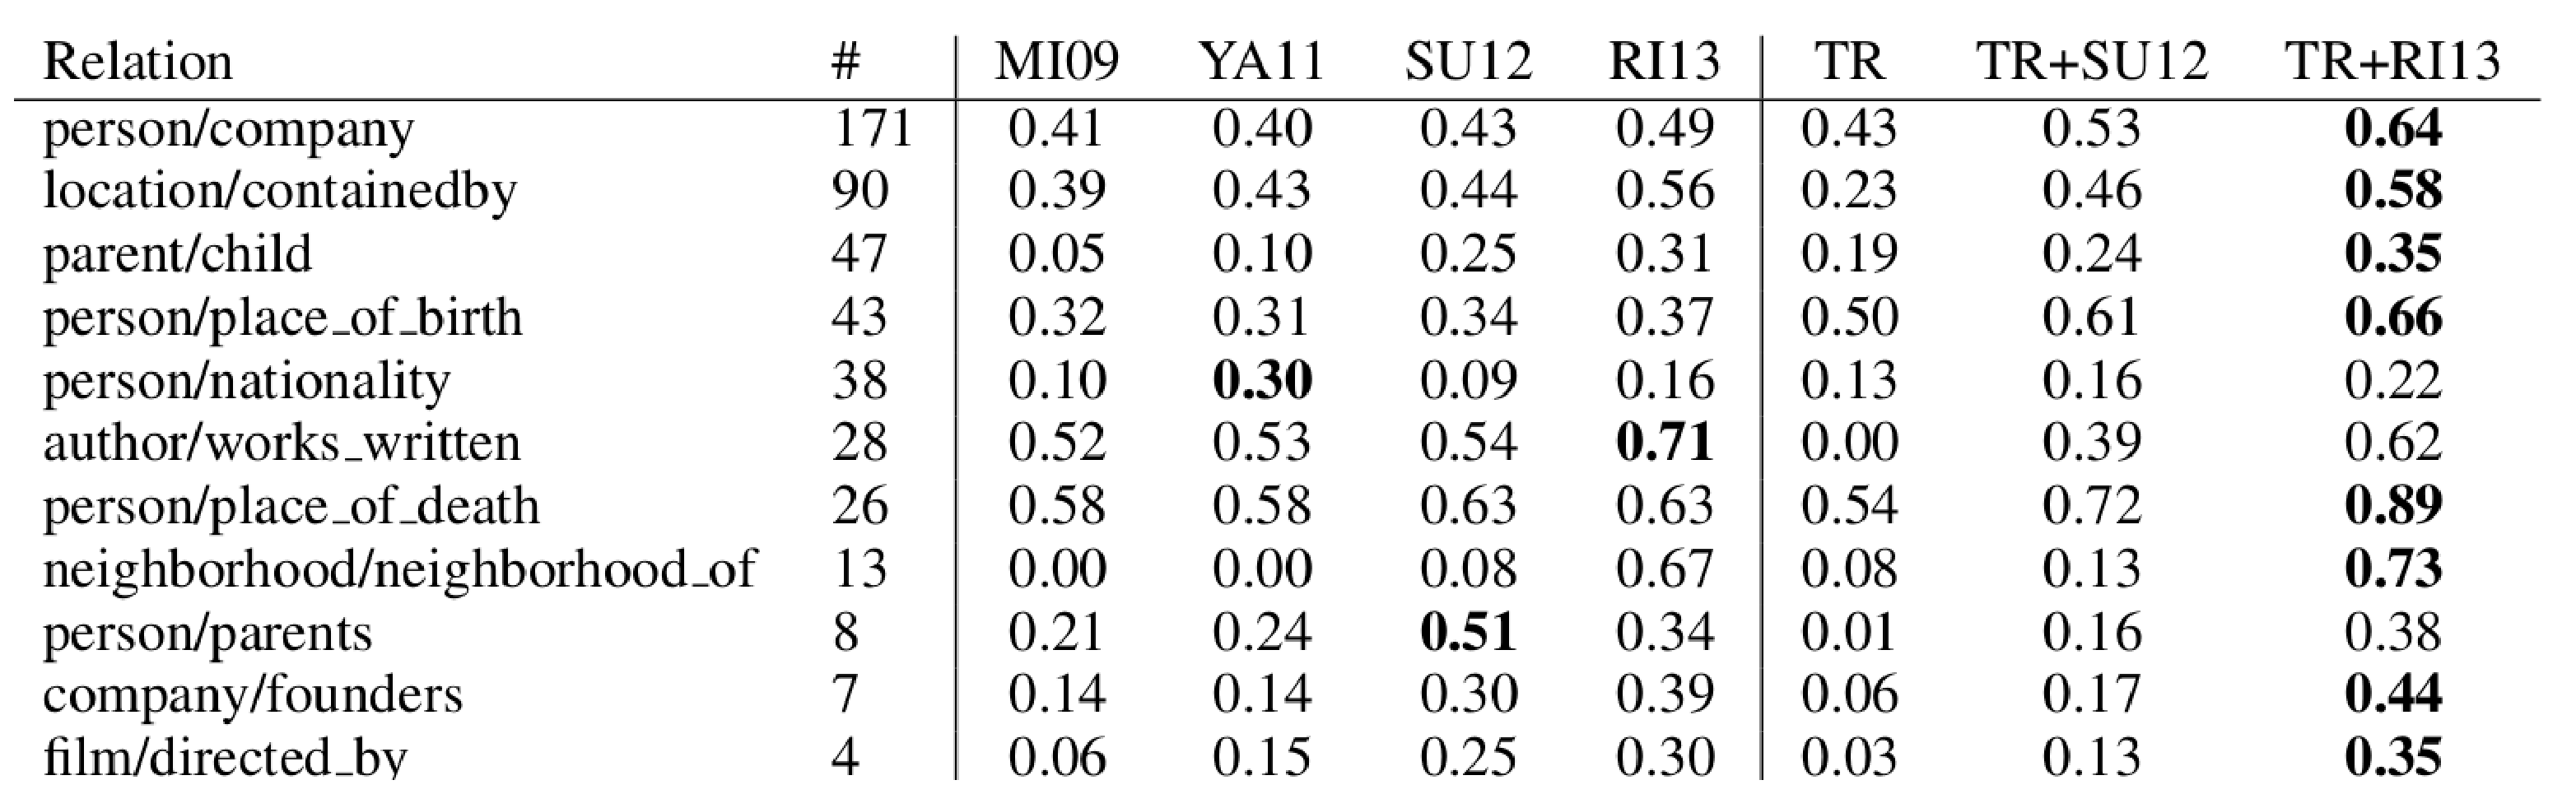
\includegraphics[width=0.8\textwidth]{WMAP}
  \end{figure}
   \end{itemize}
   \item Conclusions
   \begin{itemize}
    \item 类别信息很有效,准确率提高,实验复杂度降低
   \end{itemize}

  \end{itemize}

}
\end{document}
